\documentclass{beamer}
\usetheme{tokitex}

\usepackage{tikz}
\usepackage{graphics}
\usepackage{multirow}
\usepackage{tabto}
\usepackage{xspace}
\usepackage{amsmath}

\usepackage{tikz}
\usepackage{clrscode3e}

\usepackage[english,bahasa]{babel}
\newtranslation[to=bahasa]{Section}{Bagian}
\newtranslation[to=bahasa]{Subsection}{Subbagian}

\usepackage{listings, lstautogobble}
\usepackage{color}

\definecolor{dkgreen}{rgb}{0,0.6,0}
\definecolor{gray}{rgb}{0.5,0.5,0.5}
\definecolor{mauve}{rgb}{0.58,0,0.82}

\lstset{frame=tb,
  language=pascal,
  aboveskip=1mm,
  belowskip=1mm,
  showstringspaces=false,
  columns=fullflexible,
  keepspaces=true,
  basicstyle={\small\ttfamily},
  numbers=none,
  numberstyle=\tiny\color{gray},
  keywordstyle=\color{blue},
  commentstyle=\color{dkgreen},
  stringstyle=\color{mauve},
  breaklines=true,
  breakatwhitespace=true,
  autogobble=true
}

\usepackage{caption}
\captionsetup[figure]{labelformat=empty}

\newcommand{\progTerm}[1]{\textbf{#1}}
\newcommand{\foreignTerm}[1]{\textit{#1}}
\newcommand{\newTerm}[1]{\alert{\textbf{#1}}}
\newcommand{\emp}[1]{\alert{#1}}
\newcommand{\statement}[1]{"#1"}

% Getting tired of writing \foreignTerm all the time
\newcommand{\farray}{\foreignTerm{array}\xspace}
\newcommand{\fArray}{\foreignTerm{Array}\xspace}
\newcommand{\foverhead}{\foreignTerm{overhead}\xspace}
\newcommand{\fOverhead}{\foreignTerm{Overhead}\xspace}
\newcommand{\fsubarray}{\foreignTerm{subarray}\xspace}
\newcommand{\fSubarray}{\foreignTerm{Subarray}\xspace}
\newcommand{\fbasecase}{\foreignTerm{base case}\xspace}
\newcommand{\fBasecase}{\foreignTerm{Base case}\xspace}
\newcommand{\ftopdown}{\foreignTerm{top down}\xspace}
\newcommand{\fTopdown}{\foreignTerm{Top down}\xspace}
\newcommand{\fbottomup}{\foreignTerm{bottom up}\xspace}
\newcommand{\fBottomup}{\foreignTerm{Bottom up}\xspace}
\newcommand{\fpruning}{\foreignTerm{pruning}\xspace}
\newcommand{\fPruning}{\foreignTerm{Pruning}\xspace}

\newcommand{\fgraph}{\foreignTerm{graph}\xspace}
\newcommand{\fGraph}{\foreignTerm{Graph}\xspace}
\newcommand{\fnode}{\foreignTerm{node}\xspace}
\newcommand{\fNode}{\foreignTerm{Node}\xspace}
\newcommand{\fedge}{\foreignTerm{edge}\xspace}
\newcommand{\fEdge}{\foreignTerm{Edge}\xspace}
\newcommand{\fdegree}{\foreignTerm{degree}\xspace}
\newcommand{\fDegree}{\foreignTerm{Degree}\xspace}
\newcommand{\fadjacencylist}{\foreignTerm{adjacency list}\xspace}
\newcommand{\fAdjacencylist}{\foreignTerm{Adjacency list}\xspace}
\newcommand{\fadjacencymatrix}{\foreignTerm{adjacency matrix}\xspace}
\newcommand{\fAdjacencymatrix}{\foreignTerm{Adjacency matrix}\xspace}
\newcommand{\fedgelist}{\foreignTerm{edge list}\xspace}
\newcommand{\fEdgelist}{\foreignTerm{Edge list}\xspace}
\newcommand{\flist}{\foreignTerm{list}\xspace}
\newcommand{\fList}{\foreignTerm{List}\xspace}
\newcommand{\fgraphtraversal}{\foreignTerm{graph traversal}\xspace}
\newcommand{\fGraphtraversal}{\foreignTerm{Graph traversal}\xspace}
\newcommand{\ftree}{\foreignTerm{tree}\xspace}
\newcommand{\fTree}{\foreignTerm{Tree}\xspace}

\newcommand{\fDivideAndConquer}{\foreignTerm{Divide and Conquer}\xspace}
\newcommand{\fMergeSort}{\foreignTerm{Merge Sort}\xspace}
\newcommand{\fQuickSort}{\foreignTerm{Quicksort}\xspace}
\newcommand{\fpivot}{\foreignTerm{pivot}\xspace}
\newcommand{\fPivot}{\foreignTerm{Pivot}\xspace}
\newcommand{\fBruteForce}{\foreignTerm{Brute Force}\xspace}
\newcommand{\fCompleteSearch}{\foreignTerm{Complete Search}\xspace}
\newcommand{\fExhaustiveSearch}{\foreignTerm{Exhaustive Search}\xspace}
\newcommand{\fBinarySearch}{\foreignTerm{Binary Search}\xspace}
\newcommand{\fGreedy}{\foreignTerm{Greedy}\xspace}
\newcommand{\fGreedyChoice}{\foreignTerm{Greedy Choice}\xspace}

\newcommand{\pheap}{\progTerm{heap}\xspace}
\newcommand{\pHeap}{\progTerm{Heap}\xspace}
\newcommand{\pBinaryHeap}{\progTerm{Binary Heap}\xspace}
\newcommand{\pbinaryHeap}{\progTerm{binary heap}\xspace}

\title{Perkenalan \fGraph}
\author{Tim Olimpiade Komputer Indonesia}
\date{}

\usepackage{verbatim}
\usepackage{multicol}
\lstset{escapeinside={<@}{@>},belowskip=\baselineskip}
\definecolor{mygreen}{rgb}{0, 0.597, 0.199}

\begin{document}

\begin{frame}
\titlepage
\end{frame}

\begin{frame}
\frametitle{Pendahuluan}
Melalui dokumen ini, kalian akan:
\begin{itemize}
  \item Mengenal konsep dan terminologi \fgraph.
  \item Mengetahui jenis-jenis \fgraph.
  \item Mengenal representasi \fgraph pada pemrograman.
  \item Mengenal metode-metode yang digunakan dalam \fgraph.
\end{itemize}
\end{frame}

\begin{frame}
\frametitle{Motivasi}
\begin{itemize}
  \item Diberikan sebuah struktur kota dan jalan.
  \item Terdapat $V$ kota, dan $E$ ruas jalan.
  \item Setiap ruas jalan menghubungkan dua kota.
  \item Diberikan kota awal, tentukan berapa banyak ruas jalan paling sedikit yang perlu dilalui untuk mencapai suatu kota tujuan!
\end{itemize}
\end{frame}

\begin{frame}
\frametitle{Pertanyaan}
\begin{center}
  \large Bagaimana cara merepresentasikan struktur perkotaan dan jalan pada pemrograman?
\end{center}
\end{frame}

\section{Perkenalan Graph}
\frame{\sectionpage}

\begin{frame}
\frametitle{Mengenal \fGraph}
\fGraph adalah struktur yang terdiri dari \alert{\fnode/\foreignTerm{vertex}} dan \alert{\fedge.}\newline

\fNode direpresentasikan dengan bentuk lingkaran dan \fedge direpresentasikan dengan bentuk garis pada ilustrasi berikut:

\begin{figure}
  \centering
  \includegraphics[width=4 cm]{asset/graph.pdf}
\end{figure}
\end{frame}

\begin{frame}
\frametitle{Mengenal \fGraph (lanj.)}
\begin{itemize}
  \item \fEdge merupakan penghubung antar \fnode.
  \item \alert{\fDegree} suatu \fnode merupakan jumlah \fedge yang terhubung pada \fnode tersebut
  \item Pada contoh ilustrasi berikut, \fdegree \fnode A = 4, \fdegree \fnode B = 3, dan \fdegree \fnode C = 5.
\end{itemize}
\begin{figure}
  \centering
  \includegraphics[width=4 cm]{asset/graph.pdf}
\end{figure}
\end{frame}

\begin{frame}
\frametitle{Jenis \fGraph}
Berdasarkan hubungan antar \fnode:
\begin{itemize}
  \item \foreignTerm{Undirected} \fgraph (dua arah): \fedge dari A ke B dapat ditelusuri dari A ke B dan B ke A. 
  \item \foreignTerm{Directed} \fgraph (satu arah): \fedge dari A ke B hanya dapat ditelusuri dari dari A ke B.
\end{itemize}
\begin{figure}
  \centering
  \includegraphics[width=4 cm]{asset/unweighted-undirected.pdf}
  \ \ \ \ \ \ % If this works, this ain't stupid
  \includegraphics[width=4 cm]{asset/unweighted-directed.pdf}
  
  \foreignTerm{Undirected} dan \foreignTerm{directed} \fgraph.
\end{figure}
\end{frame}

\begin{frame}
\frametitle{Jenis \fGraph (lanj.)}
Berdasarkan bobot dari \fedge:
\begin{itemize}
  \item \foreignTerm{Unweighted} \fGraph, yaitu \fgraph dengan \fedge yang bobotnya seragam dan hanya bermakna terdapat hubungan antar \fnode.
  \item \foreignTerm{Weighted} \fGraph, yaitu \fgraph dengan \fedge yang dapat memiliki bobot berbeda-beda. Bobot pada \fedge ini bisa jadi berupa biaya, jarak, atau waktu yang harus ditempuh jika menggunakan \fedge tersebut.
\end{itemize}
\begin{figure}
  \centering
  \includegraphics[width=4 cm]{asset/unweighted-undirected.pdf}
  \ \ \ \ \ \ % If this works, this ain't stupid
  \includegraphics[width=4 cm]{asset/weighted-undirected.pdf}
  
  \foreignTerm{Unweighted} dan \foreignTerm{weighted} \fgraph.
\end{figure}
\end{frame}

\begin{frame}
\frametitle{Jenis \fGraph (lanj.)}
Tentu saja, suatu \fgraph dapat memiliki kombinasi dari sifat-sifat tersebut.

Misalnya \foreignTerm{weighted directed graph}:
\newline
\begin{figure}
  \centering
  \includegraphics[width=5 cm]{asset/weighted-directed.pdf}
\end{figure}
\end{frame}

\begin{frame}
\frametitle{Representasi \fGraph pada Pemrograman}

\begin{itemize}
  \item Dalam pemrograman, dibutuhkan sebuah struktur agar data mengenai \fgraph dapat disimpan dan diolah.
  \item Representasi yang akan kita pelajari adalah \fadjacencymatrix, \fadjacencylist, dan \fedgelist.
  \item Masing-masing representasi memiliki keuntungan dan kerugiannya.
  \item Penggunaan representasi \fgraph bergantung dengan masalah yang sedang dihadapi
\end{itemize}
\end{frame}

\begin{frame}
\frametitle{Adjacency Matrix}
\begin{itemize}
  \item Kita akan menggunakan matriks dengan ukuran $N \times N$ dengan $N$ merupakan banyaknya \fnode.
  \item Pada \foreignTerm{unweighted} \fgraph:
  \begin{itemize}
    \item Jika terdapat \fedge dari A ke B, maka $matrix[A][B] = 1$. 
    \item Jika tidak ada, maka $matrix[A][B] = 0$.
  \end{itemize}
\end{itemize}

\begin{center}
\begin{multicols}{2}
  $\begin{array}{c|cccc}
      & A & B & C & D \\ \hline
    A & 0 & 1 & 1 & 1 \\
    B & 1 & 0 & 0 & 0 \\
    C & 0 & 0 & 0 & 1 \\
    D & 0 & 0 & 0 & 0
  \end{array}$
  \break
  \begin{figure}
    \includegraphics[width=4 cm]{asset/unweighted-directed.pdf}
  \end{figure}
\end{multicols} 
\end{center}
\end{frame}

\begin{frame}
\frametitle{Adjacency Matrix (lanj.)}
\begin{itemize}
  \item Pada \foreignTerm{weighted} \fgraph:
  \begin{itemize}
    \item Jika terdapat \fedge dari A ke B dengan bobot w, maka $matrix[A][B] = w$. 
    \item Jika tidak ada, maka dapat ditulis $matrix[A][B] = \infty$.
  \end{itemize}
\end{itemize}

\begin{center}
\begin{multicols}{2}
  $\begin{array}{c|cccc}
      & A & B & C & D \\ \hline
    A & \infty & 3 & 2 & 5 \\
    B & 1 & \infty & \infty & \infty \\
    C & \infty & \infty & \infty & 8 \\
    D & \infty & \infty & \infty & \infty
  \end{array}$
  \break
  \begin{figure}
    \includegraphics[width=4 cm]{asset/weighted-directed.pdf}
  \end{figure}
\end{multicols} 
\end{center}
\end{frame}

\begin{frame}
\frametitle{Analisis Adjacency Matrix}
\begin{itemize}
  \item Pada \foreignTerm{undirected} \fgraph, \fadjacencymatrix simetris terhadap diagonalnya.
  \item Representasi ini mudah diimplementasikan.
  \item Menambah atau menghapus \fedge dapat dilakukan dalam $O(1)$.
  \item Untuk memeriksa apakah dua \fnode terhubung juga dapat dilakukan dalam $O(1)$.
  \item Untuk mendapatkan daftar tetangga dari suatu \fnode, dapat dilakukan iterasi $O(V)$, dengan $V$ adalah banyaknya \fnode.
\end{itemize}
\end{frame}

\begin{frame}
\frametitle{Kekurangan Adjacency Matrix}
\begin{itemize}
  \item Kekurangan dari representasi ini adalah boros memori.
  \item Memori yang dibutuhkan selalu $O(V^2)$, tidak dapat digunakan untuk \fgraph dengan \fnode mencapai ratusan ribu.
  \item Jika banyaknya \fedge jauh lebih sedikit dari $O(V^2)$, maka banyak memori yang terbuang.
\end{itemize}
\end{frame}

\begin{frame}
\frametitle{Adjacency List}
\begin{itemize}
  \item Merupakan salah satu alternatif representasi \fgraph.
  \item Untuk setiap \fnode, buat sebuath \flist yang berisi keterangan mengenai tetangga \fnode tersebut.
  \item Misalnya untuk \foreignTerm{unweighted} \fgraph, kita cukup menyimpan \fnode-\fnode tetangga untuk setiap \fnode.
\end{itemize}
\begin{center}
\begin{multicols}{2}
  $\begin{array}{r|l}
    A & [B, C, D] \\
    B & [A] \\
    C & [D] \\
    D & [\ ]
  \end{array}$
  \break
  \begin{figure}
    \includegraphics[width=4 cm]{asset/unweighted-directed.pdf}
  \end{figure}
\end{multicols} 
\end{center}
\end{frame}

\begin{frame}
\frametitle{Adjacency List (lanj.)}
\begin{itemize}
  \item Untuk \foreignTerm{weighted} \fgraph, kita dapat menyimpan \fnode-\fnode tetangga beserta bobotnya.
\end{itemize}
\begin{center}
\begin{multicols}{2}
  $\begin{array}{r|l}
    A & [<B,3> , <C,2>, <D,5>] \\
    B & [<A,1>] \\
    C & [<D,8>] \\
    D & [\ ]
  \end{array}$
  \break
  \begin{figure}
    \includegraphics[width=4 cm]{asset/weighted-directed.pdf}
  \end{figure}
\end{multicols} 
\end{center}
\end{frame}

\begin{frame}
\frametitle{Implementasi Adjacency List}
\begin{itemize}
  \item Kita dapat menggunakan struktur data \foreignTerm{array of lists}.
  \item Tiap \flist berisi keterangan mengenai tetangga suatu \fnode.
  \item Ukuran dari \farray merupakan $V$, yang mana $V$ merupakan banyaknya \fnode.
  \item Dengan menggunakan \flist, banyaknya memori yang digunakan untuk setiap \fnode hanya sebatas banyak tetangganya.
  \item Secara keseluruhan jika \fgraph memiliki $E$ \fedge, maka total memori yang dibutuhkan adalah $O(E)$.
\end{itemize}
\end{frame}

\begin{frame}
\frametitle{Implementasi Adjacency List (lanj.)}
\begin{itemize}
  \item \fList yang dimaksud bisa berupa \foreignTerm{Linked List} atau \foreignTerm{Resizable Array}.
  \item Bagi pengguna C++ atau Java, struktur \flist yang dapat digunakan adalah Vector atau ArrayList.
  \item Untuk pengguna C atau Pascal, struktur \foreignTerm{Linked List} perlu dibuat terlebih dahulu.
\end{itemize}
\end{frame}

\begin{frame}
\frametitle{Analisis Adjacency List}
\begin{itemize}
  \item Kompleksitas menambah \fedge adalah $O(1)$, dan menghapus adalah $O(K)$ dengan $K$ adalah banyaknya tetangga dari \fnode yang \fedge-nya dihapus.
  \item Memeriksa apakah dua \fnode terhubung oleh \fedge juga dilakukan dalam $O(K)$.
  \item Demikian juga untuk mendapatkan daftar tetangga dari \fnode, kompleksitasnya adalah $O(K)$. Perhatikan bahwa pencarian daftar tetangga ini sudah paling efisien.
\end{itemize}
\end{frame}

\begin{frame}
\frametitle{Edge List}
\begin{itemize}
  \item Sesuai namanya, kita merepresentasikan \fgraph dengan sebuah \flist.
  \item Seluruh keterangan \fedge dimasukkan kedalam \flist tersebut.
  \item Berbeda dengan \fadjacencylist yang membutuhkan \foreignTerm{array of list}, representasi ini hanya butuh sebuah \flist.
\end{itemize}
\begin{center}
\begin{multicols}{2}
  $\begin{array}{l}
    <A, B>, \\
    <A, C>, \\
    <A, D>, \\
    <B, A>, \\
    <C, D> 
  \end{array}$
  \break
  \begin{figure}
    \includegraphics[width=4 cm]{asset/unweighted-directed.pdf}
  \end{figure}
\end{multicols} 
\end{center}
\end{frame}

\begin{frame}
\frametitle{Edge List (lanj.)}
\begin{itemize}
  \item Untuk \foreignTerm{weighted} \fgraph, kita juga menyimpan bobot dari setiap \fedge.
\end{itemize}
\begin{center}
\begin{multicols}{2}
  $\begin{array}{l}
    <A, B, 3>, \\
    <A, C, 2>, \\
    <A, D, 5>, \\
    <B, A, 1>, \\
    <C, D, 8> 
  \end{array}$
  \break
  \begin{figure}
    \includegraphics[width=4 cm]{asset/weighted-directed.pdf}
  \end{figure}
\end{multicols} 
\end{center}
\end{frame}

\begin{frame}
\frametitle{Implementasi Edge List}
\begin{itemize}
  \item Untuk implementasinya, kita membutuhkan struktur data sebuah \flist (atau \farray).
  \item Jelas bahwa memori yang dibutuhkan adalah $O(E)$, dengan $E$ adalah banyaknya \fedge pada keseluruhan \fgraph.
  \newline
  \item Pada beberapa kasus, dilakukan pengurutan terhadap \fedgelist atau digunakan struktur data \foreignTerm{Binary Search Tree}, yang memungkinkan implementasinya lebih efisien.
  Namun untuk saat ini kita tidak mempelajari hal tersebut.
\end{itemize}
\end{frame}

\begin{frame}
\frametitle{Analisis Edge List}
\begin{itemize}
  \item Kompleksitas menambah \fedge adalah $O(1)$.
  \item Bergantung dari implementasi, kompleksitas menghapus \fedge dan memeriksa keterhubungan sepasang \fnode bisa berupa $O(\log{E})$ sampai $O(E)$.
  \item Demikian juga untuk mendapatkan daftar tetangga dari \fnode, kompleksitasnya bisa berkisar antara $O(\log{E} + K)$ sampai $O(E)$, dengan $K$ adalah banyaknya tetangga dari \fnode tersebut.
\end{itemize}
\end{frame}

\begin{frame}
\frametitle{Keuntungan dan Kerugian Representasi \fGraph}
Untuk \fgraph dengan $V$ \fnode dan $E$ \fedge: 
{\fontsize{9}{10}\selectfont\renewcommand{\arraystretch}{1.75}
\begin{center}
 \begin{tabular}{||r|c c c||} 
 \hline
 & \foreignTerm{Adj.Matrix} & \foreignTerm{Adj.List} & \foreignTerm{Edge List}\\
 \hline\hline
 Tambah \fedge & $O(1)$ & $O(1)$ & $O(1)$ \\ \hline
 Hapus \fedge & $O(1)$ & $O(K)$ & $O(E)$ \\ \hline
 Cek keterhubungan & $O(1)$ & $O(K)$ & $O(E)$ \\ \hline
 Daftar tetangga & $O(V)$ & $O(K)$ & $O(E)$ \\ \hline
 Kebutuhan memori & $O(V^2)$ & $O(E)$ & $O(E)$ \\ [0.5ex] 
 \hline
\end{tabular}
\end{center}
}
Dengan $K$ adalah banyaknya \fnode yang bertetangga dengan \fnode yang sedang kita periksa.
\end{frame}

%\begin{frame}[fragile]
%\frametitle{Pseudocode Representasi \fGraph}
%
%Adjacency Matrix
%\begin{lstlisting}
%  integer AdjMatrix[N][N]
%  set AdjMatrix = 0
%  
%  <@\textcolor{mygreen}{//edge dari 1 ke 4 pada undirected unweighted graph}@>
%  AdjMatrix[1][4] = 1
%  AdjMatrix[4][1] = 1
%\end{lstlisting}
%Adjacency List
%\begin{lstlisting}
%  List<integer> AdjList[N]
%  
%  <@\textcolor{mygreen}{//edge dari 1 ke 4 pada undirected unweighted graph}@>
%  AdjList[1].push(4)
%  AdjList[4].push(1)
%  
%\end{lstlisting}
%\end{frame}
%
%\begin{frame}[fragile]
%\frametitle{Pseudocode Representasi \fGraph (lanj.)}
%
%Edge List
%\begin{lstlisting}
%  List<{integer,integer}> EdgeList
%  
%  <@\textcolor{mygreen}{//edge dari 1 ke 4 pada undirected unweighted graph}@>
%  EdgeList.push({1,4})
%  
%  List<{integer,integer,integer}> WeightedList
%  
%  <@\textcolor{mygreen}{//edge dari 2 ke 3 dengan bobot 5 pada undirected graph}@>
%  WeightedList.push({2,3,5})
%\end{lstlisting}
%\end{frame}

\begin{comment}
\begin{frame}
\frametitle{Keuntungan dan Kerugian Representasi \fGraph}

\begin{itemize}
  \item Adjacency Matrix memakan lebih banyak memori. Hal ini dikarenakan adjacency matrix menyimpan keterangan dari satu node ke semua node. Sedangkan dalam adjacency list, suatu node hanya menyimpan keterangan mengenai node lain yang memiliki edge. Oleh karena itu, adjacency list lebih baik digunakan ketika edge yang terdapat tidak teralu banyak.
  \item Untuk melakukan pengecekan atau perubahan edge dari A ke B, pada adjacency matrix dapat dilakukan dengan hanya melihat dan mengubah matrix[A][B]. Sedangkan pada adjacency list, kita harus mengiterasi seluruh elemen pada list[A]
\end{itemize}
\end{frame}

\begin{frame}
\frametitle{Keuntungan dan Kerugian Representasi \fGraph (lanj.)}
\begin{itemize}
  \item Jika ada edge dari A ke B yang akan dibuang, maka pada adjacency matrix kita hanya perlu mengubah nilai Matrix[A][B]. Sedangkan pada adjacency list, harus dilakukan iterasi terlebih dahulu untuk mencari edge tersebut, lalu menghapusnya juga lebih rumit karena harus menggeser seluruh elemen setelahnya.
  \item Untuk mencari tetangga-tetangganya, maka pada adjacency matrix perlu dilakukan iterasi terhadap seluruh node yagn ada. Sementara itu, pada adjacency list hanya perlu dilakukan iterasi pada list yang isinya merupakan tetangga dari node yang bersangkutan.
\end{itemize}
\end{frame}
\end{comment}

\section{Graph Traversal}
\frame{\sectionpage}

\begin{frame}
\frametitle{\fGraph Traversal}
\begin{itemize}
  \item Representasi \fGraph saja belum berguna karena belum dapat mencari informasi mengenai suatu \fgraph
  \item \alert{\fGraph Traversal} merupakan penelusuran \fnode-\fnode pada suatu \fgraph.
\end{itemize}
\end{frame}

\begin{frame}
\frametitle{\fGraph Traversal (lanj.)}
\begin{itemize}
  \item Diberikan \fnode A dan \fnode B, apakah dari \fnode A kita dapat pergi ke \fnode B dengan \fedge yang ada?
  \item Permasalahan tersebut dapat diselesaikan menggunakan \fgraphtraversal.
  \newline
  \item Terdapat 2 metode yang dapat digunakan, yaitu \newTerm{DFS} dan \newTerm{BFS}.
\end{itemize}
\end{frame}

\begin{frame}
\frametitle{DFS: Depth-First Search}
Penelusuran dilakukan terhadap \fnode yang lebih dalam terlebih dahulu (\foreignTerm{depth-first}). 

Sebagai contoh, misal terdapat \fgraph berikut:

\begin{figure}
  \centering
  \includegraphics[width=4 cm]{asset/plain.pdf}
\end{figure}
\end{frame}

\begin{frame}
\frametitle{DFS: Depth-First Search (lanj.)}
Penelusuran secara DFS akan dilakukan dengan cara berikut:
\begin{figure}
  \centering
  \includegraphics[width=4 cm]{asset/dfs.pdf}
\end{figure}
\begin{itemize}
  \item Angka pada \fnode menunjukkan urutan \fnode tersebut dikunjungi.
  \item \fNode 1 dikunjungi pertama, \fnode 2 dikunjungi kedua, dan seterusnya).
\end{itemize}
\end{frame}

\begin{frame}
\frametitle{Penelusuran DFS}
\begin{figure}
  \centering
  \includegraphics[width=4 cm]{asset/dfs.pdf}
\end{figure}
\begin{itemize}
  \item Dapat dilihat bahwa DFS mencoba menelusuri \fnode yang dalam terlebih dahulu.
  \item \fNode yang dekat dengan \fnode pertama (seperti \fnode 7 dan 8) akan dikunjungi setelah DFS selesai mengunjungi \fnode yang lebih dalam (seperti \fnode 3, 4, dan 5)
  \item Dalam pemrograman, DFS biasa dilakukan dengan rekursi atau struktur data \foreignTerm{stack}
\end{itemize}
\end{frame}


\begin{frame}[fragile]
\frametitle{Implementasi DFS (Rekursif)}
%\begin{lstlisting}
%integer AdjMatrix[N][N]
%boolean flag[N]
%set flag = false
%flag[1] = true
%
%procedure DFS(integer currNode):
%  for i=1 to N
%    <@\textcolor{mygreen}{//check apakah ada edge dan belum pernah dikunjungi}@>
%    if AdjMatrix[currNode][i]==1 and flag[i]==false
%      flag[i] = true
%      DFS(i)
%end        
%\end{lstlisting}
Asumsikan:
\begin{itemize}
  \item Setiap \fnode dinomori dari 1 sampai $V$
  \item $adj(x)$ menyatakan himpunan tetangga dari \fnode $x$.
  \item $visit[x]$ bernilai $true$ hanya jika $x$ telah dikunjungi.
\end{itemize}
\begin{codebox}
  \Procname{$\proc{DFS}(currNode)$}
  \li \textbf{Print} "mengunjungi $currNode$"
  \li \For \textbf{each} $adjNode \in adj(currNode)$ \Do
  \li   \If \textbf{not} $visit[adjNode]$ \Then
  \li     $visit[adjNode] \gets true$
  \li     $\proc{DFS}(adjNode)$
        \End
      \End
\end{codebox}
\end{frame}

\begin{frame}[fragile]
\frametitle{Implementasi DFS (Stack)}
%\begin{lstlisting}
%integer AdjMatrix[N][N]
%boolean flag[N]
%set flag = false
%stack <integer> s
%
%s.push(1), flag[1] = true
%while s is not empty
%  integer currNode = s.top()
%  s.pop()
%  for i=1 to N
%    if AdjMatrix[currNode][i]==1 and flag[i]==false
%      flag[i] = true
%      s.push(i)
%        
%\end{lstlisting}
\begin{codebox}
  \Procname{$\proc{DFS}()$}
  \li \Comment Inisialisasi $stack$ sebagai stack kosong.
  \li $stack.push(initialNode)$
  \li $visit[initialNode] \gets true$
  \li \While \textbf{not} $stack.empty()$ \Do
  \li   $currNode \gets stack.top()$
  \li   $stack.pop()$
  \li   \textbf{Print} "mengunjungi $currNode$"
  \li   \For \textbf{each} $adjNode \in adj(currNode)$ \Do
  \li     \If \textbf{not} $visit[adjNode]$ \Then
  \li       $visit[adjNode] \gets true$
  \li       $stack.push(adjNode)$
          \End
        \End
      \End
\end{codebox}
\end{frame}

\begin{frame}
\frametitle{BFS: Breadth-First Search}
Penelusuran \fnode pada \fgraph dilakukan lapis demi lapis. 

Semakin dekat suatu \fnode dengan \fnode awal, \fnode tersebut akan dikunjungi terlebih dahulu. 

\begin{figure}
  \centering
  \includegraphics[width=4 cm]{asset/bfs.pdf}
\end{figure}
\end{frame}

\begin{frame}
\frametitle{Penelusuran BFS}
\begin{figure}
  \centering
  \includegraphics[width=4 cm]{asset/bfs.pdf}
\end{figure}
\begin{itemize}
  \item Angka pada gambar menunjukkan urutan \fnode tersebut dikunjungi.
  \item Dalam pemrograman, BFS biasa diimplementasikan dengan bantuan struktur data \foreignTerm{queue}.
\end{itemize}
\end{frame}

\begin{frame}[fragile]
\frametitle{Implementasi BFS}
%BFS membutuhkan bantuan struktur data queue. Berikut adalah potongan kodenya\newline
%\begin{lstlisting}
%integer AdjMatrix[N][N]
%boolean flag[N]
%set flag = false
%queue <integer> q
%
%q.push(1), flag[1] = true
%while q is not empty
%  integer currNode = q.front()
%  q.pop()
%  for i=1 to N
%    if AdjMatrix[currNode][i]==1 and flag[i]==false
%      flag[i] = true
%      q.push(i)
%        
%\end{lstlisting}
\begin{codebox}
  \Procname{$\proc{BFS}()$}
  \li \Comment Inisialisasi $queue$ sebagai queue kosong.
  \li $queue.push(initialNode)$
  \li $visit[initialNode] \gets true$
  \li \While \textbf{not} $queue.empty()$ \Do
  \li   $currNode \gets queue.front()$
  \li   $queue.pop()$
  \li   \textbf{Print} "mengunjungi $currNode$"
  \li   \For \textbf{each} $adjNode \in adj(currNode)$ \Do
  \li     \If \textbf{not} $visit[adjNode]$ \Then
  \li       $visit[adjNode] \gets true$
  \li       $queue.push(adjNode)$
          \End
        \End
      \End
\end{codebox}
\end{frame}

\begin{frame}
\frametitle{Analisis Kompleksitas}
\begin{itemize}
  \item Baik DFS maupun BFS sama-sama mengunjungi setiap \fnode tepat satu kali, dengan memanfaatkan seluruh \fedge.
  \item Kompleksitas dari kedua metode adalah:
  \begin{itemize}
    \item $O(V^2)$, jika digunakan \fadjacencymatrix.
    \item $O(V + E)$, jika digunakan \fadjacencylist.
    \newline
  \end{itemize}
  \item Penggunaan DFS atau BFS dapat disesuaikan dengan persoalan yang dihadapi.
\end{itemize}
\end{frame}

\begin{frame}
\frametitle{Contoh Permasalahan (lanj.)}
Pak Dengklek tinggal di kota A. Suatu hari, beliau ingin pergi ke kota B. Terdapat beberapa ruas jalan yang menghubungkan kota-kota dalam negara tempat beliau tinggal. Namun karena sudah tua, Pak Dengklek ingin melewati sesedikit mungkin ruas jalan untuk sampai ke kota B.
\newline\newline
Diberikan informasi mengenai struktur kota dan ruas jalan, tentukan berapa banyak ruas jalan yang perlu beliau lewati untuk pergi dari kota A ke kota B!
\end{frame}

\begin{frame}
\frametitle{Solusi}
\begin{itemize}
  \item Permasalahan ini dapat diselesaikan dengan BFS. 
  \item Karena sifat BFS yang menelusuri \fnode lapis demi lapis, maka dapat disimpulkan jika suatu \fnode dikunjungi, maka jarak yang ditempuh dari awal sampai \fnode tersebut pasti jarak terpendek.
  \item Hal ini selalu benar untuk segala \foreignTerm{unweighted} \fgraph, BFS selalu menemukan \foreignTerm{shortest path} dari suatu \fnode ke seluruh \fnode lainnya.
\end{itemize}
\end{frame}

\begin{frame}[fragile]
\frametitle{Implementasi Solusi}
%\begin{lstlisting}
%integer AdjMatrix[N][N] , A , B , jarak = -1
%queue < (integer,integer) > q
%<@\textcolor{mygreen}{//Queue menyimpan node yang dikunjungi dan jarak dari A}@>
%q.push({A,0}), flag[A] = true
%while q is not empty
%  (integer,integer) currNode = q.front()
%  q.pop()
%  <@\textcolor{mygreen}{//Cek jika telah sampai di kota B}@>
%  if currNode.first == B
%    jarak = currNode.second, break
%  for i=1 to N
%    if AdjMatrix[currNode.first][i]==1 and flag[i]==false
%      flag[i] = true
%      q.push({i,currNode.second+1})
%if jarak!=-1
%  print jarak
%else
%  print 'Tidak dapat ke kota B'    
%\end{lstlisting}
\begin{codebox}
  \Procname{$\proc{shortestPath}(A, B)$}
  \li \Comment Inisialisasi $queue$ sebagai queue kosong.
  \li \Comment Inisialisasi array $visitTime$ dengan -1.
  \li $queue.push(A)$
  \li $visitTime[A] \gets 0$
  \li \While \textbf{not} $queue.empty()$ \Do
  \li   $currNode \gets queue.front()$
  \li   $queue.pop()$
  \li   \For \textbf{each} $adjNode \in adj(currNode)$ \Do
  \li     \Comment Jika $adjNode$ belum pernah dikunjungi...
  \li     \If $visitTime[adjNode] \isequal -1$ \Then
  \li       $visitTime[adjNode] \gets visitTime[currNode] + 1$
  \li       $queue.push(adjNode)$
          \End
        \End
      \End
  \li \Return $visitTime[B]$
\end{codebox}
\end{frame}

\section{Macam-Macam Graph}
\frame{\sectionpage}

\begin{frame}
\frametitle{Macam-Macam Graph}
\begin{itemize}
  \item Terdapat \fGraph yang memiliki suatu karakteristik khusus, sehingga penyelesaian masalah yang melibatkan \fgraph ini dapat memanfaatkan karakter tersebut.
  \item Contoh macam-macam \fgraph adalah \newTerm{Tree}, \newTerm{Directed Acyclic Graph}, dan \newTerm{Bipartite Graph}.
  \item Kali ini kita akan menyinggung \fTree dan \foreignTerm{Directed Acyclic Graph}.
\end{itemize}
\end{frame}

\begin{frame}
\frametitle{Tree}
\begin{itemize}
  \item \fTree merupakan bentuk khusus dari \fgraph.
  \item Seluruh \fnode pada \ftree terhubung (tidak ada \fnode yang tidak dapat dikunjungi dari \fnode lain) dan tidak terdapat \alert{cycle}.
  \item Jumlah \fedge dalam sebuah \ftree pasti $V-1$, dengan $V$ adalah banyaknya \fnode.
\end{itemize}
\begin{center}
  \includegraphics[width=3.5 cm]{asset/plain.pdf}
\end{center}
\end{frame}

\begin{frame}
\frametitle{Contoh Tree}
\includegraphics[width=3.5 cm]{asset/not-tree.pdf}
\hspace{\fill}
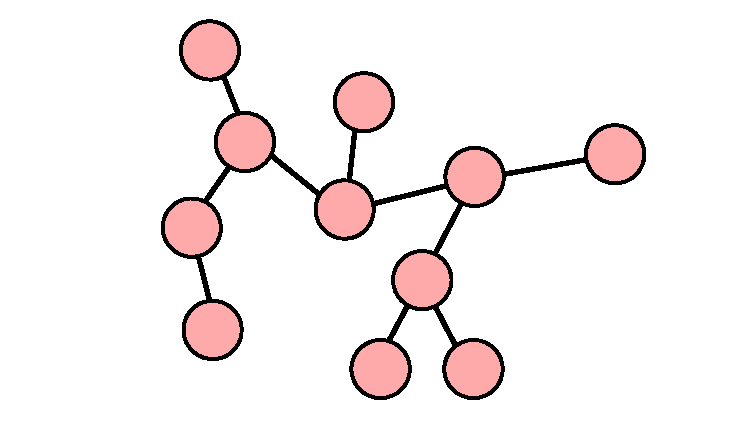
\includegraphics[width=4 cm]{asset/tree.pdf}
\newline\newline
Gambar kiri bukan \ftree karena memiliki \foreignTerm{cycle}, sedangkan gambar kanan merupakan \ftree. 
\end{frame}

\begin{frame}
\frametitle{Directed Acyclic \fGraph}
\begin{itemize}
  \item \foreignTerm{Directed Acyclic \fGraph (DAG)} merupakan bentuk khusus dari \foreignTerm{directed} \fgraph.
  \item DAG tidak memiliki \alert{cycle}.
  \item Berbeda dengan \ftree yang mana setiap \fnode harus dapat dikunjungi dari \fnode lainnya, sifat tersebut tidak berlaku pada DAG.
\end{itemize}
\begin{center}
  \includegraphics[width=4 cm]{asset/dag.pdf}
\end{center}
\end{frame}

\begin{frame}
\frametitle{Contoh Directed Acyclic \fGraph}
\includegraphics[width=4 cm]{asset/dag.pdf}
\hspace{\fill}
\includegraphics[width=5 cm]{asset/not-dag.pdf}
\newline\newline
Pada gambar di atas, gambar kiri merupakan DAG, sedangkan gambar kanan bukan DAG karena memiliki \foreignTerm{cycle}.
\end{frame}

\begin{frame}
\frametitle{Penutup}
\begin{itemize}
  \item Hampir setiap kompetisi pasti memiliki soal yang bertemakan \fgraph.
  \item Mampu menguasai dasar penyelesaian masalah \fgraph menjadi kemampuan penting dalam dunia kompetisi.
  \item Selamat berlatih dengan soal-soal yang diberikan.
\end{itemize}
\end{frame}

\end{document}
